Auf der 100-Meter-Bahn der KS Im Lee wird ein Roboter getestet. Er wird auf der Startlinie gesetzt und beschleunigt schnell in Richtung Ziellinie. Während der Fahrt folgt die Bewegung des Roboters der Bewegungsgleichung
\[
    s(t) = \frac{1}{4}t^2
\]
Das ist so zu verstehen, dass der Roboter nach t Sekunden die Strecke $s\left(t\right)=\frac{1}{4}t^2$ in Metern zurückgelegt hat. Wir denken uns entlang der Bahn ein Messband ausgelegt, sodass wir immer die Position des Roboters in Meter nach dem Startpunkt ablesen können.
\begin{enumerate}
    \item 	Skizzieren Sie den Graphen der Funktion $s\left(t\right)$ im Bereich $0\le t\le8$
    \begin{figure}[H]
        \centering
        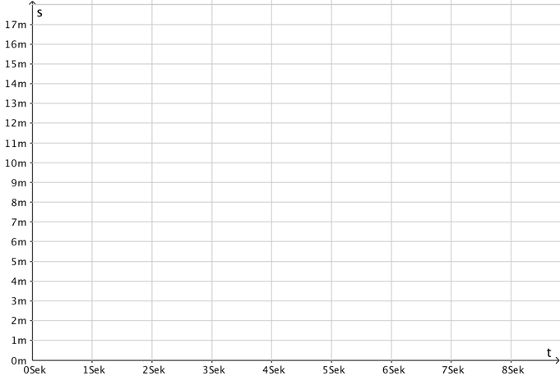
\includegraphics[scale = 0.7]{im/RoboterDiagramm.png}
    \end{figure}
    \item 	Welche Position lesen wir auf dem Messband 2 Sekunden nach dem Start ab? Und welche Position 6 Sekunden nach dem Start? Markieren Sie die entsprechenden Punkte auf dem Graphen.
	\item Welche Distanz legt der Roboter zwischen dem Zeitpunkt $t=2$ und $t=6$ zurück? Wie gross ist demnach die Durchschnittsgeschwindigkeit $\bar{v}$ in $\frac{m}{s}$ zwischen den beiden genannten Zeitpunkten?
	\item Zur Berechnung von $\bar{v}$ haben Sie so etwas wie „obsi/vorwärts“ gerechnet. Von welcher Geraden ist $\bar{v}$ die Steigung? Zeichnen Sie die Gerade in den Graphen oben ein.
	\item Berechnen Sie die Durchschnittsgeschwindigkeit des Roboters zwischen den Zeitpunkten $t=2$ und $t=2+\mathrm{\Delta t}$ für $\mathrm{\Delta t}=4,\ 3,\ 2,\ 1,\ 0.5$.
	\item Bisher war immer die Rede von einer durchschnittlichen Geschwindigkeit im Intervall $[2,\ 2+\mathrm{\Delta t}]$. Wie schnell aber fährt der Roboters genau zum Zeitpunkt $t=2$? Das heisst, schätzen Sie seine Momentangeschwindigkeit 
	$v\left(2\right)$.
	\item Von welcher Gerade ist die $v\left(2\right)$ die Steigung? Zeichnen Sie die Gerade in den Graphen oben.
	\item Was ist die Momentangeschwindigkeit des Roboters zum Zeitpunkt $t=8$?
\end{enumerate}